\documentclass[12pt]{article}
\usepackage[utf8]{inputenc}
\usepackage{tgbonum}
\usepackage[a4paper, total={7in, 10in}]{geometry}
\usepackage{graphicx}
\usepackage{minted}
\title{Lab Assignment 6}
\author{Akshat Mittal - 20107}
\date{July 2021}
\begin{document}
\maketitle
\vspace{7mm}
\textbf{Contents}
\vspace{7mm}
\begin{enumerate}
    \item Addresses of array elements
    \item Use of refrerencing and dereferencing operators
    \item Circular swapping
    \item Finding Factorial
    \item Vowels and consonants
    \item Sorting using pointers
    \item Sum of elements of an array
    \item Reversing the string
    \item Reversing individual characters of string
    \item No. of words in a string
    \item Comparing two strings
    \item no. of alphabets, numbers, special characters
    \item Copying one string into another
    \item To find maximum occuring character in a string
    \item Checking for substring
    \item Library Functions of string.h
    \item Conversion of lowercase to uppercase
    \item Fetching a substring
    \item Replacing a word
    \item Deleting vowels from a string
\end{enumerate}

\newpage
\section{}
\subsection{Code}
\inputminted{c}{q1.c}
\subsection{Output}
\begin{figure}[h]
    \centering
    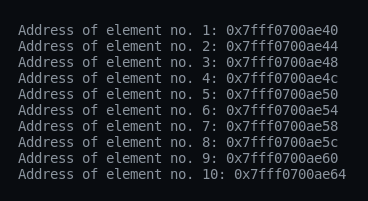
\includegraphics{1.png}
\end{figure}

\newpage
\section{}
\subsection{Code}
\inputminted{c}{q2.c}
\subsection{Output}
\begin{figure}[h]
    \centering
    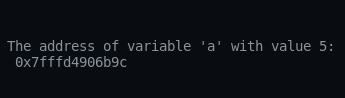
\includegraphics{2.png}
\end{figure}

\newpage
\section{}
\subsection{Code}
\inputminted{c}{q3.c}
\subsection{Output}
\begin{figure}[h]
    \centering
    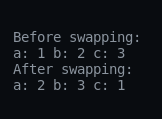
\includegraphics[width=0.5\textwidth]{3.png}
\end{figure}

\newpage
\section{}
\subsection{Code}
\inputminted{c}{q4.c}
\subsection{Output}
\begin{figure}[h]
    \centering
    
\includegraphics[width=0.9\textwidth]{4.png}
\end{figure}

\newpage
\section{}
\subsection{Code}
\inputminted{c}{q5.c}
\subsection{Output}
\begin{figure}[h]
    \centering
    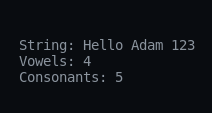
\includegraphics[width=0.7\textwidth]{5.png}
\end{figure}

\newpage
\section{}
\subsection{Code}
\inputminted{c}{q6.c}
\newpage
\subsection{Output}
\begin{figure}[h]
    \centering
    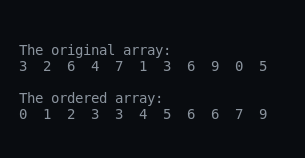
\includegraphics[width=0.75\textwidth]{6.png}
\end{figure}

\newpage
\section{}
\subsection{Code}
\inputminted{c}{q7.c}
\subsection{Output}
\begin{figure}[h]
    \centering
    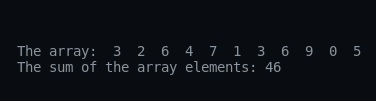
\includegraphics[width=0.75\textwidth]{7.png}
\end{figure}

\newpage
\section{}
\subsection{Code}
\inputminted{c}{q8.c}
\subsection{Output}
\begin{figure}[h]
    \centering
    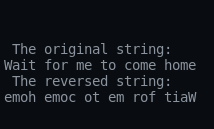
\includegraphics[width=0.6\textwidth]{8.png}
\end{figure}
\newpage
\section{}
\subsection{Code}
\inputminted{c}{q9.c}
\subsection{Output}
\begin{figure}[h]
    \centering
    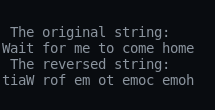
\includegraphics[width=0.5\textwidth]{9.png}
\end{figure}
\newpage
\section{}
\subsection{Code}
\inputminted{c}{q10.c}
\subsection{Output}
\begin{figure}[h]
    \centering
    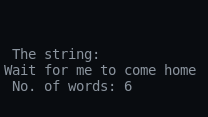
\includegraphics[width=0.5\textwidth]{ 10.png}
\end{figure}
\newpage
\section{}
\subsection{Code}
\inputminted{c}{q11.c}
\subsection{Output}
\begin{figure}[h]
    \centering
    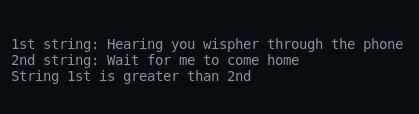
\includegraphics{11.png}
\end{figure}

\newpage
\section{}
\subsection{Code}
\inputminted{c}{q12.c}
\subsection{Output}
\begin{figure}[h]
    \centering
    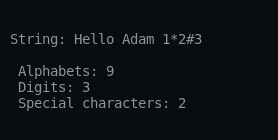
\includegraphics{12.png}
\end{figure}

\newpage
\section{}
\subsection{Code}
\inputminted{c}{q13.c}
\subsection{Output}
\begin{figure}[h]
    \centering
    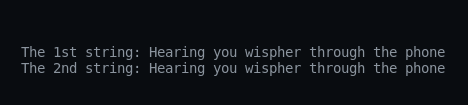
\includegraphics{13.png}
\end{figure}

\newpage
\section{}
\subsection{Code}
\inputminted{c}{q14.c}
\subsection{Output}
\begin{figure}[h]
    \centering
    
\includegraphics[width=0.62\textwidth]{14.png}
\end{figure}

\newpage
\section{}
\subsection{Code}
\inputminted{c}{q15.c}
\subsection{Output}
\begin{figure}[h]
    \centering
    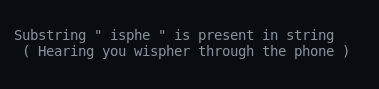
\includegraphics[width=1.0\textwidth]{15.png}
\end{figure}

\newpage
\section{}
\subsection{Code}
\inputminted{c}{q16.c}
\subsection{Output}
\begin{figure}[h]
    \centering
    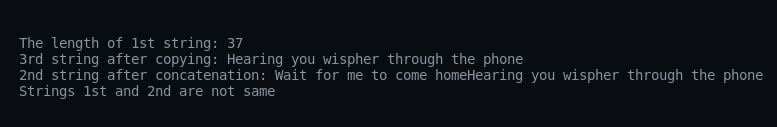
\includegraphics[width=1.0\textwidth]{16.png}
\end{figure}

\newpage
\section{}
\subsection{Code}
\inputminted{c}{q17.c}
\subsection{Output}
\begin{figure}[h]
    \centering
    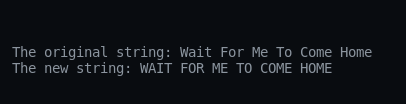
\includegraphics[width=0.75\textwidth]{17.png}
\end{figure}

\newpage
\section{}
\subsection{Code}
\inputminted{c}{q18.c}
\subsection{Output}
\begin{figure}[h]
    \centering
    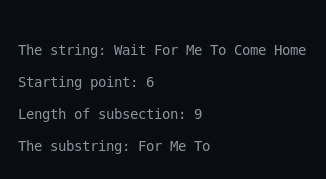
\includegraphics{18.png}
\end{figure}
\newpage
\section{}
\subsection{Code}
%\inputminted{c}{Q19.c}
\subsection{Output}
\begin{figure}[h]
    \centering
    %\includegraphics[width=0.5\textwidth]{19.png}
\end{figure}
\newpage
\section{}
\subsection{Code}
\inputminted{c}{q20.c}
\subsection{Output}
\begin{figure}[h]
    \centering
    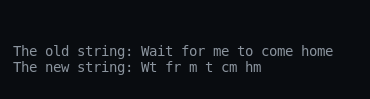
\includegraphics[width=0.6\textwidth]{20.png}
\end{figure}

\end{document}